\documentclass[a4paper,12pt]{article}
\usepackage{amsmath}
\usepackage{amsfonts}
\usepackage{amssymb}
\usepackage{geometry}
\usepackage{graphicx}
\usepackage[T1]{fontenc}  % Kodowanie czcionki z polskimi znakami
\usepackage[utf8]{inputenc}  % Kodowanie znaków UTF-8
\usepackage{polski}  % Obsługa polskich znaków
\geometry{margin=1in}

\title{Raport z zadania NUM5 \\ \large Analiza metod iteracyjnych dla układu równań liniowych}
\author{Bartosz Satoła}
\date{28 listopada 2024}

\begin{document}

\maketitle

\tableofcontents
\newpage

\section{Opis ćwiczenia}

Celem ćwiczenia było rozwiązanie układu równań liniowych opisanego równaniem:
\[
A \cdot x = b,
\]
gdzie macierz \(A\) ma specyficzną strukturę:
\[
A =
\begin{bmatrix}
d & 0.5 & 0.1 & & & \\
0.5 & d & 0.5 & 0.1 & & \\
0.1 & 0.5 & d & 0.5 & 0.1 & \\
& \ddots & \ddots & \ddots & \ddots & \\
& & 0.1 & 0.5 & d & 0.5 \\
& & & 0.1 & 0.5 & d
\end{bmatrix},
\]
a wektor \(b\) to \([1, 2, 3, \ldots, N]^T\) o długości \(N = 200\).

Macierz \(A\) jest macierzą pięciodiagonalną, co oznacza, że wartości różne od zera znajdują się wyłącznie na głównej przekątnej oraz na dwóch przekątnych powyżej i poniżej. Taka struktura pozwala na zoptymalizowane przechowywanie oraz efektywne obliczenia, ponieważ większość elementów macierzy to zera.

W zadaniu użyto dwóch metod iteracyjnych: \textbf{metody Jacobiego} oraz \textbf{metody Gaussa-Seidela}. Zadanie polegało na:
\begin{itemize}
    \item Porównaniu obu metod pod względem szybkości zbieżności i dokładności.
    \item Analizie wpływu parametru \(d\) na zbieżność metod.
    \item Sprawdzeniu, czy macierz \(A\) spełnia warunki zbieżności, takie jak dominacja diagonalna i dodatnia określoność.
    \item Graficznej prezentacji błędu w kolejnych iteracjach.
    \item Zbadaniu przypadków, w których procedury iteracyjne mogą nie być zbieżne.
\end{itemize}

W szczególności metoda Gaussa-Seidela wymaga, aby macierz była \textbf{dodatnio określona}, co oznacza, że dla dowolnego niezerowego wektora \(x\) zachodzi:
\[
x^T A x > 0.
\]
Dodatnia określoność jest niezbędna do zapewnienia stabilności i zbieżności tej metody iteracyjnej. W przypadku metody Jacobiego, koniecznym warunkiem zbieżności jest dominacja diagonalna macierzy \(A\), czyli:
\[
|a_{ii}| > \sum_{j \neq i} |a_{ij}|, \quad \forall i.
\]
Oba te warunki zostały szczegółowo przeanalizowane w ramach ćwiczenia.

\section{Wstęp teoretyczny}

\subsection{Macierz układu}

Macierz \(A\) w zadaniu ma strukturę pięciodiagonalną, co oznacza, że wartości różne od zera znajdują się na:
\begin{itemize}
    \item głównej przekątnej (\(d\)),
    \item pierwszej przekątnej powyżej i poniżej (\(0.5\)),
    \item drugiej przekątnej powyżej i poniżej (\(0.1\)).
\end{itemize}

Taka macierz jest rzadka, co pozwala na zoptymalizowane przechowywanie i obliczenia. W zadaniu zastosowano wstęgową reprezentację macierzy, ograniczając pamięć do przechowywania tylko pięciu wstęg.

\subsection{Zbieżność metod iteracyjnych}

Dla zbieżności metod iteracyjnych, takich jak Jacobi i Gauss-Seidel, konieczne są odpowiednie warunki na macierz \(A\):
\begin{itemize}
    \item \textbf{Dominacja diagonalna:} Metoda Jacobiego wymaga, aby macierz była dominująca diagonalnie, co oznacza, że każdy element głównej przekątnej jest większy (w sensie bezwzględnym) od sumy wartości z innych kolumn tego samego wiersza:
    \[
    |a_{ii}| > \sum_{j \neq i} |a_{ij}|, \quad \forall i.
    \]
    \item \textbf{Dodatnia określoność:} Metoda Gaussa-Seidela wymaga, aby macierz była dodatnio określona. Oznacza to, że dla każdego niezerowego wektora \(x\) zachodzi:
    \[
    x^T A x > 0.
    \]
    Dodatnia określoność jest również gwarantowana, jeśli wszystkie wartości własne macierzy \(A\) są dodatnie.
\end{itemize}

\subsection{Metody iteracyjne}

Metody iteracyjne, takie jak Jacobi i Gauss-Seidel, wykorzystują przybliżone obliczenia, tworząc sekwencję wektorów \(x^{(k)}\), która zbiega do dokładnego rozwiązania \(x\). Poniżej opisano kluczowe różnice między tymi metodami.

\subsubsection{Metoda Jacobiego}

Metoda Jacobiego dzieli macierz \(A\) na:
\[
A = D + R,
\]
gdzie:
\begin{itemize}
    \item \(D\) to macierz diagonalna (zawiera elementy głównej przekątnej),
    \item \(R = A - D\) to macierz zawierająca pozostałe elementy (spoza głównej przekątnej).
\end{itemize}

Iteracyjny schemat Jacobiego wygląda następująco:
\[
x^{(k+1)} = D^{-1} \cdot (b - R \cdot x^{(k)}),
\]
co dla każdego elementu \(x_i\) można zapisać jako:
\[
x_i^{(k+1)} = \frac{1}{a_{ii}} \left( b_i - \sum_{j \neq i} a_{ij} x_j^{(k)} \right).
\]

\paragraph{Zalety:}
\begin{itemize}
    \item Prosta implementacja.
    \item Możliwość łatwej równoległości obliczeń, ponieważ każdy \(x_i^{(k+1)}\) jest obliczany niezależnie.
\end{itemize}

\paragraph{Wady:}
\begin{itemize}
    \item Wolniejsza zbieżność w porównaniu do metody Gaussa-Seidela.
    \item Wrażliwość na uwarunkowanie macierzy; wymaga dominacji diagonalnej dla zbieżności.
\end{itemize}

\subsubsection{Metoda Gaussa-Seidela}

Metoda Gaussa-Seidela różni się od Jacobiego tym, że natychmiast wykorzystuje nowo obliczone wartości \(x_i^{(k+1)}\) w bieżącej iteracji:
\[
x_i^{(k+1)} = \frac{1}{a_{ii}} \left( b_i - \sum_{j=1}^{i-1} a_{ij} x_j^{(k+1)} - \sum_{j=i+1}^N a_{ij} x_j^{(k)} \right).
\]

\paragraph{Zalety:}
\begin{itemize}
    \item Szybsza zbieżność dzięki natychmiastowemu wykorzystaniu nowych wartości.
    \item Mniejsza liczba iteracji w porównaniu do metody Jacobiego.
\end{itemize}

\paragraph{Wady:}
\begin{itemize}
    \item Brak możliwości łatwej równoległości obliczeń.
    \item Wymaga, aby macierz była dodatnio określona, co ogranicza zakres jej zastosowania.
\end{itemize}

\subsection{Podsumowanie oczekiwanych wyników}

\begin{itemize}
    \item Dla \(d = 2, 3, 4\): Macierz \(A\) spełnia warunki dominacji diagonalnej i dodatniej określoności. Obie metody powinny być zbieżne, przy czym Gauss-Seidel powinien osiągać zbieżność szybciej.
    \item Dla \(d = 0.5\): Macierz \(A\) nie spełnia warunków dominacji diagonalnej i dodatniej określoności. W takim przypadku metody iteracyjne mogą być rozbieżne.
\end{itemize}

\section{Omówienie programu}

Program został zaprojektowany w języku Python z uwzględnieniem optymalizacji dla macierzy pięciodiagonalnych. Implementacja obejmuje następujące kluczowe elementy:

\begin{enumerate}
    \item \textbf{Tworzenie macierzy pięciodiagonalnej:}
    \begin{itemize}
        \item Macierz \(A\) jest przechowywana w formacie wstęgowym jako tablica \(5 \times N\), gdzie:
        \begin{itemize}
            \item Główna przekątna (\(d\)) znajduje się w środkowym wierszu tablicy.
            \item Pierwsza nadprzekątna (\(0.5\)) i pierwsza podprzekątna (\(0.5\)) są zapisywane odpowiednio w wierszach powyżej i poniżej głównej przekątnej.
            \item Druga nadprzekątna (\(0.1\)) i druga podprzekątna (\(0.1\)) są przechowywane w skrajnych wierszach tablicy.
        \end{itemize}
        \item Taka reprezentacja zmniejsza zużycie pamięci z \(O(N^2)\) do \(O(5N)\).
    \end{itemize}
    
    \item \textbf{Operacje na macierzy wstęgowej:}
    \begin{itemize}
        \item Operacje mnożenia macierzy przez wektor zostały zoptymalizowane, aby korzystać tylko z istotnych wstęg macierzy. 
        \item Dzięki temu złożoność obliczeniowa operacji została zredukowana do \(O(N)\).
    \end{itemize}
    
    \item \textbf{Metody iteracyjne:}
    \begin{itemize}
        \item \textbf{Metoda Jacobiego:} Implementacja iteracji korzysta wyłącznie z danych z wstęg. Nowe wartości \(x^{(k+1)}\) są obliczane w całości na podstawie wartości \(x^{(k)}\) z poprzedniej iteracji.
        \item \textbf{Metoda Gaussa-Seidela:} Wartości \(x^{(k+1)}\) są aktualizowane w miejscu, co pozwala na natychmiastowe wykorzystanie nowych wyników w bieżącej iteracji.
        \item W obu metodach normy \( \infty \) różnic między kolejnymi przybliżeniami są obliczane w celu monitorowania zbieżności.
    \end{itemize}
    
    \item \textbf{Obliczanie dokładnego rozwiązania:}
    \begin{itemize}
        \item Dla porównania wyników metod iteracyjnych zastosowano funkcję \texttt{numpy.linalg.solve}, która wykorzystuje eliminację Gaussa do dokładnego rozwiązania układu.
    \end{itemize}
    
    \item \textbf{Wizualizacja wyników:}
    \begin{itemize}
        \item Wyniki są prezentowane graficznie w postaci wykresów przedstawiających zależność błędu (w normie \( \infty \)) od liczby iteracji.
        \item Porównano szybkość zbieżności obu metod dla różnych wartości parametru \(d\).
    \end{itemize}
\end{enumerate}

\section{Przedstawienie wyników}

Wyniki zostały przeanalizowane dla różnych wartości parametru \(d\). Poniżej przedstawiono rezultaty dla kilku wartości \(d\). Dla każdej z tych wartości został rozwiązany stosowny układ równań. Jednak z racji na długość rozwiązania, nie zostało ono zamieszczone w każdym przypadku. W celu zobaczenia pełnego rozwiązania należy uruchomić program \texttt{main.py}. 

Istotny jest fakt, że w przypadkach \(d = 2, 3, 4\) rozwiązanie zgadzało się z tym, zwróconym przez funkcję \texttt{numpy.linalg.solve}, z kolei dla \(d = 0.5\) żadna z metod nie zwróciła poprawnego rozwiązania, co zresztą widać na wykresie.


\begin{itemize}
    \item \textbf{Przypadek \(d = 2\):}
    \begin{itemize}
        \item Wyniki potwierdzają zbieżność obu metod iteracyjnych.
        \item Metoda Gaussa-Seidela osiągnęła zbieżność szybciej niż metoda Jacobiego.
    \end{itemize}

    \noindent\makebox[\textwidth]{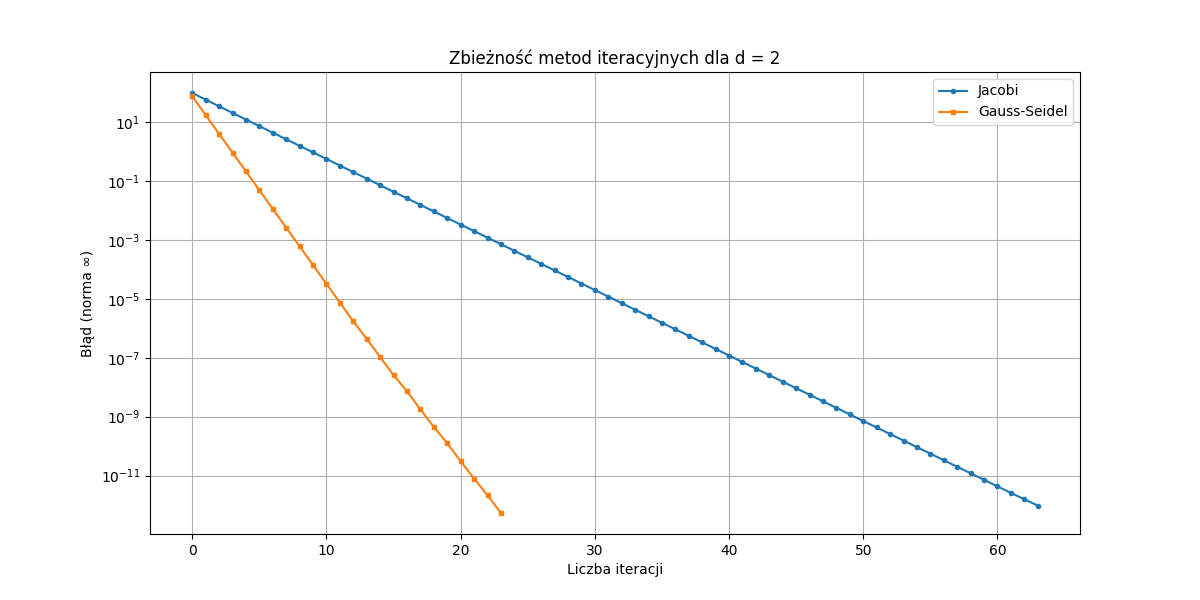
\includegraphics[width=\textwidth]{wykres_d2.png}}
    \begin{center}
        \textit{Rysunek: Zbieżność metod iteracyjnych dla \(d = 2\).}
    \end{center}

    \noindent\textbf{Wyniki obliczeń:}
    \begin{verbatim}
    --- d = 2 ---
    Rozwiązanie dokładne:
    [ 0.29582854  0.62922177  0.9373203   1.24982028  1.5625551   1.87499564
      ...
      60.65766947 81.77387418]
    Rozwiązanie Jacobiego:
    [ 0.29582854  0.62922177  0.9373203   1.24982028  1.5625551   1.87499564
      ...
      60.65766947 81.77387418]
    Rozwiązanie Gaussa-Seidela:
    [ 0.29582854  0.62922177  0.9373203   1.24982028  1.5625551   1.87499564
      ...
      60.65766947 81.77387418]
    Norma końcowego błędu Jacobiego: 9.521272659185342e-13
    Norma końcowego błędu Gaussa-Seidela: 5.329070518200751e-13
    \end{verbatim}


    \item \textbf{Przypadek \(d = 3\):}
    \begin{itemize}
        \item Obie metody iteracyjne były zbieżne.
        \item Metoda Gaussa-Seidela wymagała mniejszej liczby iteracji niż metoda Jacobiego.
    \end{itemize}

    \noindent\makebox[\textwidth]{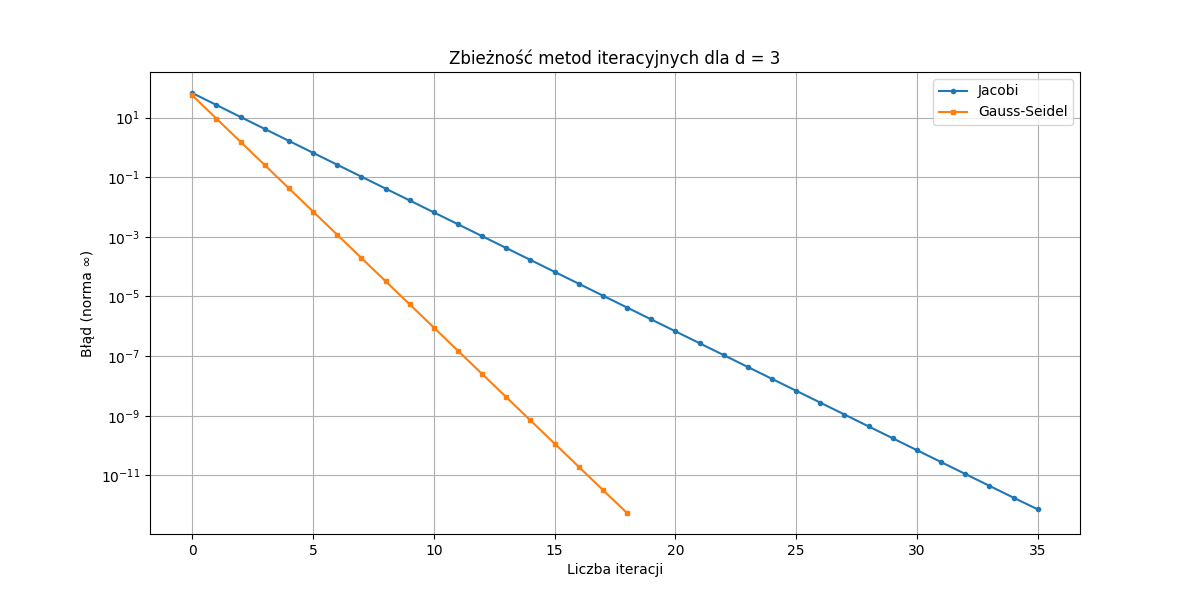
\includegraphics[width=\textwidth]{wykres_d3.png}}
    \begin{center}
        \textit{Rysunek: Zbieżność metod iteracyjnych dla \(d = 3\).}
    \end{center}

    \item \textbf{Przypadek \(d = 4\):}
    \begin{itemize}
        \item Wartość \(d = 4\) zapewniła najszybszą zbieżność obu metod.
        \item Metoda Gaussa-Seidela ponownie była bardziej efektywna.
    \end{itemize}

    \noindent\makebox[\textwidth]{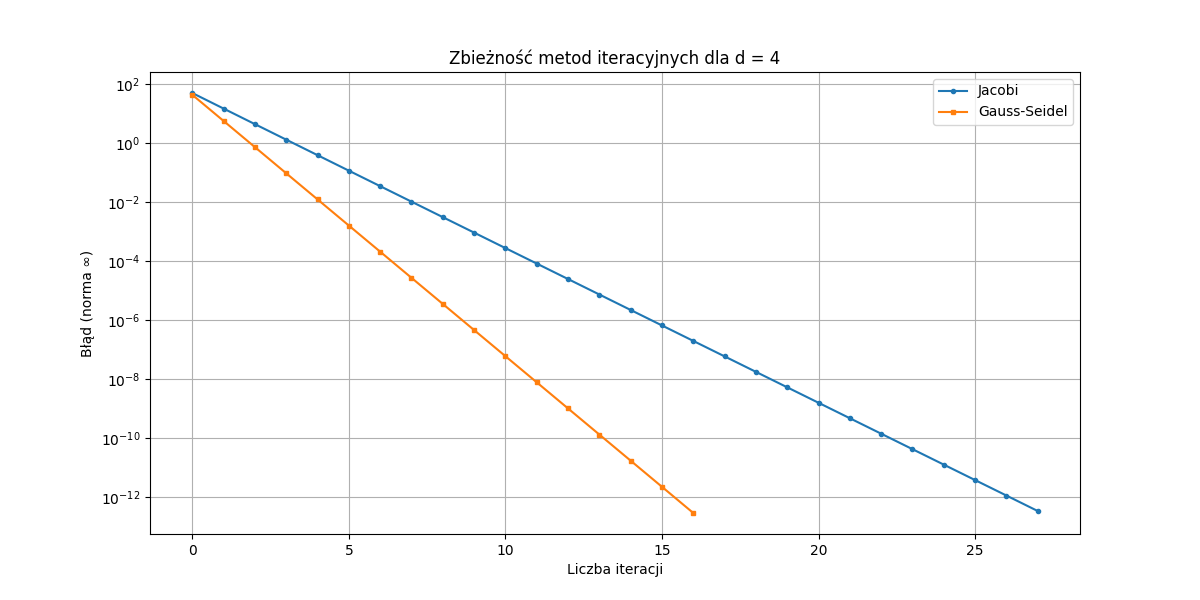
\includegraphics[width=\textwidth]{wykres_d4.png}}
    \begin{center}
        \textit{Rysunek: Zbieżność metod iteracyjnych dla \(d = 4\).}
    \end{center}

    \item \textbf{Przypadek \(d = 0.5\):}
    \begin{itemize}
        \item Brak zbieżności obu metod iteracyjnych.
        \item Wartość \(d = 0.5\) nie spełniała warunków dominacji diagonalnej i dodatniej określoności.
    \end{itemize}

    \noindent\makebox[\textwidth]{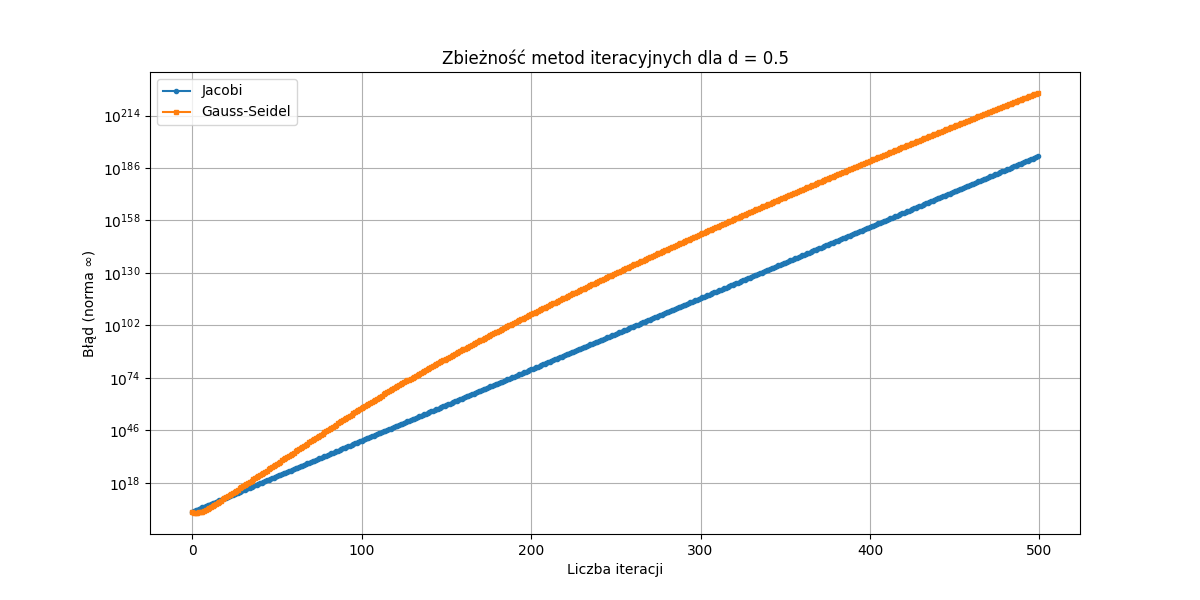
\includegraphics[width=\textwidth]{wykres_d05.png}}
    \begin{center}
        \textit{Rysunek: Brak zbieżności metod iteracyjnych dla \(d = 0.5\).}
    \end{center}

    \noindent\textbf{Wyniki obliczeń:}
    \begin{verbatim}
    --- d = 0.5 ---
    Rozwiązanie dokładne:
    [ 141.24845112 -131.71774961  -37.65350752 ... 133.42318318 203.54886074
      -56.39125369]
    Rozwiązanie Jacobiego:
    [-8.56453537e+189 -1.58795653e+190 -2.33769802e+190 ... -7.73792000e+190
     -4.17710200e+190]
    Rozwiązanie Gaussa-Seidela:
    [ 1.41696879e+164 -2.75594844e+164 -3.49255503e+164 ... -1.80735246e+224
      2.73736239e+224]
    Norma końcowego błędu Jacobiego: 1.462299035462992e+192
    Norma końcowego błędu Gaussa-Seidela: 1.0725946057871731e+226
    \end{verbatim}

\end{itemize}




\section{Wnioski}

Na podstawie przeprowadzonej analizy wyników metod iteracyjnych Jacobiego i Gaussa-Seidela można sformułować następujące wnioski:

\subsection{Skuteczność metod iteracyjnych}

\begin{itemize}
    \item \textbf{Metoda Jacobiego:}
    \begin{itemize}
        \item Skutecznie znajduje rozwiązanie układu równań liniowych, gdy macierz \(A\) spełnia warunek dominacji diagonalnej.
        \item Ze względu na niezależność obliczeń poszczególnych elementów \(x_i^{(k+1)}\), metoda jest odpowiednia dla równoległego przetwarzania obliczeń, co czyni ją użyteczną w dużych układach z zastosowaniem nowoczesnych technologii obliczeniowych.
        \item Wolniejsza zbieżność w porównaniu do metody Gaussa-Seidela sprawia, że wymaga większej liczby iteracji, co może zwiększać czas obliczeń w mniej wydajnych środowiskach.
        \item Nie wymaga, aby macierz \(A\) była dodatnio określona, co pozwala stosować ją w szerszym zakresie układów równań liniowych.
    \end{itemize}
    
    \item \textbf{Metoda Gaussa-Seidela:}
    \begin{itemize}
        \item Charakteryzuje się szybszą zbieżnością dzięki natychmiastowemu wykorzystaniu nowo obliczonych wartości \(x_i^{(k+1)}\) w trakcie iteracji.
        \item Wymaga, aby macierz była dodatnio określona, co ogranicza jej zastosowanie w układach, które nie spełniają tego warunku.
        \item Skutecznie znajduje rozwiązanie układu równań liniowych w przypadkach, gdy macierz \(A\) spełnia zarówno warunek dominacji diagonalnej, jak i dodatniej określoności.
        \item Brak równoległości w obliczeniach sprawia, że jest mniej efektywna w systemach wielordzeniowych lub rozproszonych, ale dobrze sprawdza się w tradycyjnych środowiskach obliczeniowych.
    \end{itemize}
\end{itemize}

\subsection{Zastosowanie metod iteracyjnych}

\begin{itemize}
    \item \textbf{Przypadki dobrze uwarunkowane:} 
    \begin{itemize}
        \item Dla \(d = 2, 3, 4\) macierz \(A\) spełnia warunki dominacji diagonalnej i dodatniej określoności, co pozwala obu metodom iteracyjnym osiągnąć zbieżność.
        \item Metoda Gaussa-Seidela była bardziej efektywna w tych przypadkach, osiągając zbieżność szybciej niż Jacobi.
        \item Metoda Jacobiego wymagała większej liczby iteracji, ale również wykazała zbieżność, co potwierdza jej użyteczność w szerokim zakresie układów.
    \end{itemize}

    \item \textbf{Przypadki źle uwarunkowane:}
    \begin{itemize}
        \item Dla \(d = 0.5\) macierz \(A\) nie spełniała warunku dominacji diagonalnej ani dodatniej określoności, co uniemożliwiło zbieżność obu metod iteracyjnych.
        \item W takich przypadkach obie metody nie są stabilne, a iteracje prowadzą do rosnących błędów, co potwierdza konieczność sprawdzania warunków zbieżności przed zastosowaniem metod iteracyjnych.
    \end{itemize}
\end{itemize}

\subsection{Znaczenie wartości \(d\)}

\begin{itemize}
    \item Wyższe wartości \(d\) (\(d \geq 2\)) poprawiają dominację diagonalną macierzy \(A\), co pozytywnie wpływa na stabilność i szybkość zbieżności metod iteracyjnych.
    \item Dla mniejszych wartości \(d\), takich jak \(d = 0.5\), brak dominacji diagonalnej i dodatniej określoności prowadzi do braku zbieżności. Pokazuje to, że parametry macierzy mają kluczowe znaczenie dla skuteczności metod iteracyjnych.
\end{itemize}

\subsection{Ogólne wnioski}

\begin{itemize}
    \item Metody iteracyjne Jacobiego i Gaussa-Seidela są skuteczne w przypadku dużych układów równań liniowych z dobrze uwarunkowanymi macierzami rzadkimi, takimi jak macierze pięciodiagonalne analizowane w tym zadaniu.
    \item Wybór metody iteracyjnej powinien uwzględniać właściwości macierzy:
    \begin{itemize}
        \item Metoda Jacobiego jest bardziej elastyczna i mniej restrykcyjna, ale wolniejsza.
        \item Metoda Gaussa-Seidela jest bardziej efektywna, ale wymaga spełnienia dodatkowych warunków, takich jak dodatnia określoność.
    \end{itemize}
\end{itemize}


\end{document}
